\chapter{Philosophie et Fondements de l'Investigation Numérique}

\epigraph{« La technique n'est jamais seulement technique. Elle redéfinit l'humain et son rapport au monde. »}{- Bernard Stiegler}

\section*{Prologue: Au-Delà de la Technique}
L'investigation numérique dépasse largement le cadre technique auquel on la réduit souvent. Elle constitue aujourd'hui une discipline philosophique à part entière, interrogeant les fondements de la vérité, de la confiance et de la justice à l'ère numérique. Ce chapitre introductif explore les dimensions épistémologiques, éthiques et ontologiques de cette pratique essentielle à notre société digitale.

\section{La Société Numérique: Nouveau Terrain de l'Être}
\subsection{La Transformation Numérique de l'Existence}
Notre époque vit une mutation ontologique fondamentale: l'être humain ne se définit plus seulement par sa présence physique mais également par son existence numérique. Cette \textbf{digitalité} devient une dimension constitutive de l'identité contemporaine, créant un \textbf{double numérique} qui échappe partiellement à son origine humaine.

\begin{itemize}
\item \textbf{Ontologie numérique}: L'être numérique comme extension de l'être physique
\item \textbf{Phénoménologie des données}: La trace numérique comme manifestation d'existence
\item \textbf{Métaphysique digitale}: Nouveaux modes d'être et de relation
\end{itemize}

\subsection{Le Paradoxe de la Transparence}
Notre société fait face à un paradoxe fondamental: la quête de transparence numérique entre en tension avec le droit à l'intimité. L'investigateur numérique opère à cette intersection délicate, devenant le gardien de l'équilibre entre vérité et vie privée.

\section{Épistémologie de la Preuve Numérique}
\subsection{De la Preuve Matérielle à la Preuve Numérique}
La nature de la preuve subit une transformation radicale:

\begin{table}[H]
\centering
\begin{tabular}{p{6cm}p{6cm}}
\hline
\textbf{Preuve traditionnelle} & \textbf{Preuve numérique} \\
\hline
Matérialité tangible & Immatérialité des bits \\
Stabilité physique & Volatilité et mutabilité \\
Authenticité par l'objet & Authenticité par la chaîne de confiance \\
Temporalité linéaire & Temporalité multidimensionnelle \\
\hline
\end{tabular}
\caption{Transition épistémologique de la preuve}
\end{table}

\subsection{La Crise de la Vérité Numérique}
L'ère numérique engendre une crise de la vérité sans précédent:
\begin{itemize}
\item \textbf{Manipulation algorithmique}: Les deepfakes et autres technologies brouillent la frontière vrai/faux
\item \textbf{Érosion de l'autorité épistémique}: Multiplication des sources de "vérité"
\item \textbf{Fragmentation du réel}: Versions multiples de la réalité coexistent
\end{itemize}

L'investigateur numérique devient ainsi un \textbf{archiviste du réel}, chargé de préserver l'intégrité de la mémoire collective.

\section{Fondements Mathématiques et Théoriques}
\subsection{Théorie de l'Information et Entropie}
La mathématique de l'investigation numérique puise ses fondements dans la théorie de l'information de Shannon:

\[
H(X) = -\sum_{i=1}^{n} P(x_i) \log_2 P(x_i)
\]

Cette équation d'entropie devient la pierre angulaire de l'analyse numérique, permettant de:
\begin{itemize}
\item Mesurer l'incertitude informationnelle
\item Détecter des anomalies par divergence entropique
\item Évaluer la compressibilité des données comme indicateur de régularité
\end{itemize}

\subsection{Théorie des Graphes et Relations}
L'analyse relationnelle repose sur la théorie des graphes, modélisant les interactions sociales et techniques:

\[
G = (V, E) \quad \text{où} \quad V = \text{ensembles de sommets}, E = \text{ensembles d'arêtes}
\]

Cette modélisation permet de révéler des structures cachées et des patterns comportementaux.

\subsection{Théorie du Chaos et Sensibilité Aux Conditions Initiales}
L'investigation numérique opère dans des systèmes complexes où de minuscules alterations peuvent avoir des conséquences considérables:

\[
\delta(t) \approx \delta(0) e^{\lambda t}
\]

Cette sensibilité aux conditions initiales rend la préservation de l'intégrité des preuves absolument cruciale.

\section{La Révolution Quantique: Changement de Paradigme}
\subsection{Épistémologie Pré-Quantique vs Post-Quantique}
La révolution quantique ne représente pas seulement une évolution technique mais un changement paradigmatique complet:

\begin{table}[H]
\centering
\begin{tabular}{p{6cm}p{6cm}}
\hline
\textbf{Paradigme pré-quantique} & \textbf{Paradigme post-quantique} \\
\hline
Déterminisme classique & Probabilisme quantique \\
Localité & Non-localité \\
Certitude cryptographique & Incertitude quantique \\
Vérité binaire & Superposition des états \\
\hline
\end{tabular}
\caption{Révolution paradigmatique quantique}
\end{table}

\subsection{Implications Philosophiques du Quantique}
La mécanique quantique introduit des concepts philosophiques radicaux:
\begin{itemize}
\item \textbf{Non-localité}: L'information transcende l'espace traditionnel
\item \textbf{Intrication}: Corrélations défiant la causalité classique
\item \textbf{Superposition}: Multiplicité des états simultanés
\item \textbf{Observateur participatif}: L'observation affecte le système observé
\end{itemize}

Ces concepts remettent en cause nos notions traditionnelles de réalité et de vérité.
\section{Le Paradoxe de l'Authenticité Invisible}
\subsection{Théorisation et Origines}
Le \textbf{paradoxe de l'authenticité invisible}, théorisé dans l'article fondateur \textit{Exploring ZK-NR} (ePrint 2025/1138), représente une avancée conceptuelle majeure dans l'épistémologie de la preuve numérique. Ce paradoxe capture la tension fondamentale entre:

\begin{itemize}
\item La \textbf{nécessité de prouver} l'authenticité et l'intégrité des preuves numériques
\item L'\textbf{exigence de confidentialité} et de protection de la vie privée
\item L'\textbf{impératif d'opposabilité} juridique des éléments numériques
\end{itemize}

\subsection{Formulation du Paradoxe}
Le paradoxe s'énonce ainsi: 

\emph{« Plus une preuve numérique est authentique et vérifiable, plus elle tend à révéler d'informations sur son contenu et son origine, compromettant ainsi la confidentialité. Inversement, plus une preuve préserve la confidentialité, plus son authenticité devient difficile à établir de manière certaine. »}

Mathématiquement, ce paradoxe peut s'exprimer comme une relation d'incertitude:

\[
\Delta A \cdot \Delta C \geq \hbar_{num}
\]

Où:
\begin{itemize}
\item $\Delta A$ représente l'incertitude sur l'authenticité
\item $\Delta C$ représente l'incertitude sur la confidentialité
\item $\hbar_{num}$ est la constante numérique fondamentale, analogue à la constante de Planck
\end{itemize}

\subsection{Implications Philosophiques}
\subsubsection{Épistémologie de la Preuve Voilée}
Le paradoxe soulève des questions profondes sur la nature de la connaissance:
\begin{itemize}
\item Peut-on \textbf{savoir} qu'une preuve est authentique sans \textbf{connaître} son contenu?
\item Comment fonder la \textbf{confiance} dans ce qui reste \textbf{invisible}?
\item La \textbf{vérité} peut-elle exister sous forme cryptée, accessible seulement par vérification sans divulgation?
\end{itemize}

\subsubsection{Ontologie de la Preuve Numérique}
Le paradoxe transforme notre conception de la preuve:
\begin{itemize}
\item La preuve n'est plus un \textbf{objet} à examiner mais un \textbf{processus} à vérifier
\item L'authenticité devient une \textbf{propriété relationnelle} plutôt qu'intrinsèque
\item La \textbf{vérification} remplace l'\textbf{examen} comme mode d'accès à la vérité
\end{itemize}

\subsection{Résolution par les Protocoles ZK-NR}
Les protocoles Zero-Knowledge Non-Repudiation (ZK-NR) offrent une résolution pratique à ce paradoxe en permettant:

\begin{align*}
\textbf{Vérification} &\without \textbf{Divulgation} \\
\textbf{Confiance} &\without \textbf{Transparence} \\
\textbf{Preuve} &\without \textbf{Révélation}
\end{align*}

\subsection{Implications pour l'Investigation Numérique}
\subsubsection{Nouveau Paradigme Investigatif}
L'investigator doit désormais maîtriser:
\begin{itemize}
\item La \textbf{cryptographie vérifiable} comme outil d'enquête
\item L'\textbf{épistémologie des preuves cryptées}
\item La \textbf{jurimétrie des preuves zero-knowledge}
\end{itemize}

\subsubsection{Transformation des Pratiques}
\begin{itemize}
\item La \textbf{collecte} de preuves devient \textbf{chiffrement certifié}
\item L'\textbf{analyse} devient \textbf{vérification cryptographique}
\item La \textbf{conservation} devient \textbf{préservation de l'intégrité cryptographique}
\end{itemize}

\subsection{Perspectives Existentielles}
Le paradoxe de l'authenticité invisible nous confronte à des questions existentielles fondamentales:

\begin{quote}
« Dans un monde où la vérité peut être cryptée, vérifiable mais invisible, que signifie vraiment "connaître"? Comment fonder la justice sur des preuves dont le contenu reste voilé? »
\end{quote}

Ce paradoxe nous invite à repenser non seulement nos techniques d'investigation, mais aussi nos conceptions profondes de la vérité, de la confiance et de la justice à l'ère numérique.

\subsection{Intégration dans le Trilemme CRO}
Le paradoxe de l'authenticité invisible s'intègre parfaitement dans le framework du Trilemme CRO en révélant pourquoi l'optimisation simultanée des trois axes (Confidentialité, Fiabilité, Opposabilité) est fondamentalement impossible, et comment les protocoles ZK-NR permettent d'approcher cet idéal tout en reconnaissant les limites imposées par le paradoxe.

\begin{figure}[H]
\centering
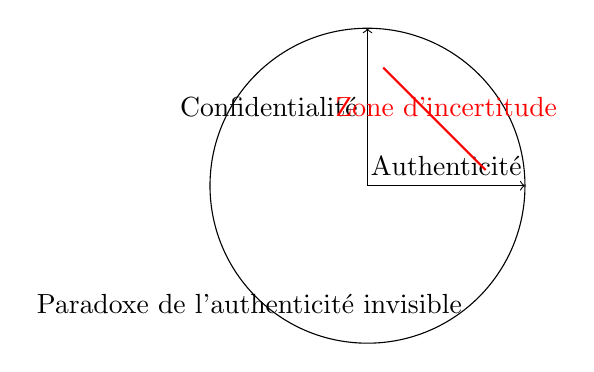
\begin{tikzpicture}
\draw (0,0) circle (2cm);
\draw[->] (0,0) -- (2,0) node[midway,above] {Authenticité};
\draw[->] (0,0) -- (0,2) node[midway,left] {Confidentialité};
\draw[red, thick] (1.5,0.2) -- (0.2,1.5);
\node[red] at (1,1) {Zone d'incertitude};
\node at (-1.5,-1.5) {Paradoxe de l'authenticité invisible};
\end{tikzpicture}
\caption{Représentation graphique du paradoxe}
\end{figure}

\section{Éthique et Responsabilité de l'Investigateur}
\subsection{L'Investigateur comme Philosophe-Praticien}
L'investigateur numérique moderne endosse un rôle triple:
\begin{enumerate}
\item \textbf{Archéologue du digital}: Exhume et préserve les traces numériques
\item \textbf{Épistémologue pratique}: Évalue la fiabilité des preuves numériques
\item \textbf{Éthicien appliqué}: Navigue les dilemmes moraux du numérique
\end{enumerate}

\subsection{Le Trilemme Éthique Fondamental}
Tout investigator doit résoudre en permanence le trilemme éthique suivant:
\begin{itemize}
\item \textbf{Transparence} vs \textbf{Vie privée}
\item \textbf{Efficacité} vs \textbf{Proportionalité}
\item \textbf{Innovation} vs \textbf{Responsabilité}
\end{itemize}

\subsection{La Chartre de l'Investigateur Numérique}
\begin{enumerate}
\item Je préserverai l'intégrité de la preuve above all
\item Je respecterai la dignité numérique des personnes
\item Je reconnaîtrai les limites de ma connaissance
\item Je travaillerai pour la vérité, pas pour la conviction
\item Je me souviendrai que derrière chaque donnée, il y a l'humain
\end{enumerate}

\section{Ontologie de la Trace Numérique}
\subsection{La Trace Comme Phénomène Existential}
La trace numérique n'est pas simple donnée mais manifestation d'existence:
\begin{itemize}
\item \textbf{Être-par-la-trace}: La trace comme mode d'être au monde numérique
\item \textbf{Intentionalité numérique}: Les traces comme révélatrices d'intention
\item \textbf{Temporalité digitale}: Le temps numérique comme dimension plurielle
\end{itemize}

\subsection{Herméneutique des Données}
L'interprétation des données nécessite une approche herméneutique:
\begin{itemize}
\item \textbf{Cercle herméneutique}: Compréhension des parties par le tout et réciproquement
\item \textbf{Préjugés algorithmiques}: Reconnaissance des biais d'interprétation
\item \textbf{Fusion des horizons}: Intégration des perspectives technique et humaine
\end{itemize}

\section{Vers une Éthique Post-Quantique}
\subsection{Les Nouveaux Impératifs Catégoriques}
À l'ère post-quantique, de nouveaux impératifs émergent:
\begin{itemize}
\item \textbf{Agis de telle sorte que les preuves que tu produis puissent résister à l'épreuve quantique}
\item \textbf{Considère l'impact de tes investigations sur les générations futures}
\item \textbf{Préserve la possibilité de l'oubli dans un monde de mémoire parfaite}
\end{itemize}

\subsection{L'Investigation Comme Praxis de Liberté}
L'investigation numérique bien comprise devient une praxis de liberté:
\begin{itemize}
\item Elle protège contre l'arbitraire en documentant le réel
\item Elle permet la reddition des comptes dans une société complexe
\item Elle préserve la mémoire collective contre l'effacement
\item Elle équilibre le pouvoir par la transparence
\end{itemize}

\section*{Conclusion: La Voie de l'Investigateur}
L'investigation numérique n'est pas une simple technique mais une voie philosophique et éthique. Elle demande autant de sagesse que de compétence, autant d'humilité que de détermination. Dans un monde où le numérique redéfinit constamment les frontières du réel et du possible, l'investigator devient le gardien de l'intégrité informationnelle, le garant de la vérité dans un monde de simulations.

\medskip

\noindent\textbf{Pour l'apprenant}: Souviens-toi que chaque décision technique que tu prendras aura des implications philosophiques. Chaque preuve que tu traiteras portera en elle une part de vérité humaine. Ta responsabilité dépasse la maîtrise technique pour embrasser une éthique complète de la pratique.

\medskip

\noindent\textbf{Notre devise}: « Savoir pour préserver, préserver pour servir, servir avec intégrité. »

\begin{figure}[H]
\centering
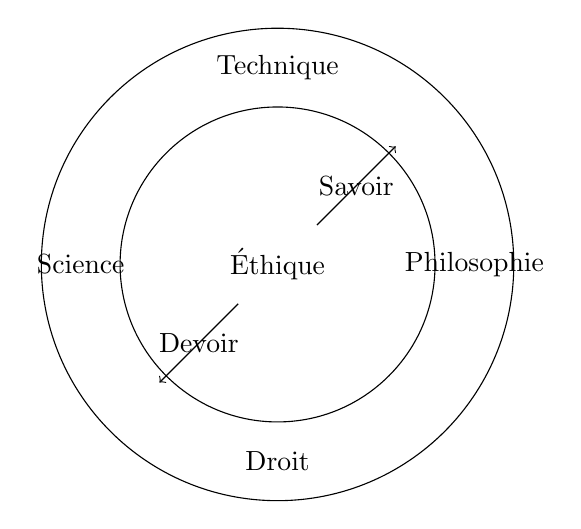
\begin{tikzpicture}
\draw (0,0) circle (2cm);
\draw (0,0) circle (3cm);
\node at (0,0) {Éthique};
\node at (0,2.5) {Technique};
\node at (0,-2.5) {Droit};
\node at (2.5,0) {Philosophie};
\node at (-2.5,0) {Science};
\draw[->] (0.5,0.5) -- (1.5,1.5);
\node at (1,1) {Savoir};
\draw[->] (-0.5,-0.5) -- (-1.5,-1.5);
\node at (-1,-1) {Devoir};
\end{tikzpicture}
\caption{L'investigation numérique à l'intersection des disciplines}
\end{figure}